% ОПЫТ №15 § 82. Закон сохранения импульса. Упругий и неупругий удар (опыт с маятниками)
\sloppy
\documentclass[14pt,a4paper,oneside]{extarticle}	% Размер основного шрифта и формата листа
\usepackage{xltxtra}						% Используется для вывода логотипа XeLaTeX
\usepackage{xunicode}						% Кодировка документа
\usepackage{polyglossia}					% Загружает пакет многоязыковой верстки
\newfontfamily\russianfont{Book Antiqua}
%\setmainfont{Liberation Serif}						% Основной шрифт текста
\setmainfont{Book Antiqua}
\setdefaultlanguage{russian}				% Основной язык текста
\setotherlanguage{english}					% Дополнительный язык текста
\linespread{1}							% Межстрочный интервал выбран полуторным
\usepackage[left=2.5cm,
right=1.5cm,vmargin=2.5cm]{geometry} % Отступы по краям листа
\bibliographystyle{ugost2008}

\usepackage{xcolor}
\usepackage{hyperref}
% Цвета для гиперссылок
\definecolor{linkcolor}{HTML}{359B08} % цвет ссылок
\definecolor{urlcolor}{HTML}{799B03} % цвет гиперссылок
\hypersetup{pdfstartview=FitH,  linkcolor=linkcolor,urlcolor=urlcolor, colorlinks=true}

%---------------------------%
%---- Пакеты расширений ----%
%---------------------------%
\usepackage{xcolor}
\usepackage{hyperref}
% Цвета для гиперссылок
\definecolor{linkcolor}{HTML}{359B08} % цвет ссылок
\definecolor{urlcolor}{HTML}{799B03} % цвет гиперссылок
\hypersetup{pdfstartview=FitH,  linkcolor=linkcolor,urlcolor=urlcolor, colorlinks=true}


\usepackage{verbatim,indentfirst}
\usepackage{cite,enumerate,float}
\usepackage{amsmath,amssymb,amsthm,amsfonts}

%---------------------------%
%--- Вставка иллюстраций ---%
%---------------------------%
\usepackage{graphicx}
\usepackage{subfigure}
%\graphicspath{{Images/}}
\usepackage{fontspec}

\begin{document}
%	\pagestyle{empty} %  выключаенм нумерацию
	
	%\setcounter{page}{3}% Нумерация начинается с третьей страницы
	%\renewcommand{\contentsname}{\center{Содержание}}
	%\tableofcontents
	
	\begin{center}
		%\addcontentsline{toc}{section}{Опыт 15. Закон сохранения импульса. Упругий и неупругий удар (опыт с маятниками)}
		\subsection*{Упругий и неупругий удар}
	\end{center}
	
	\begin{figure}[H] 	% Окружение для вставки иллюстрации
		\centering 	
		% Выравнивание по центру
		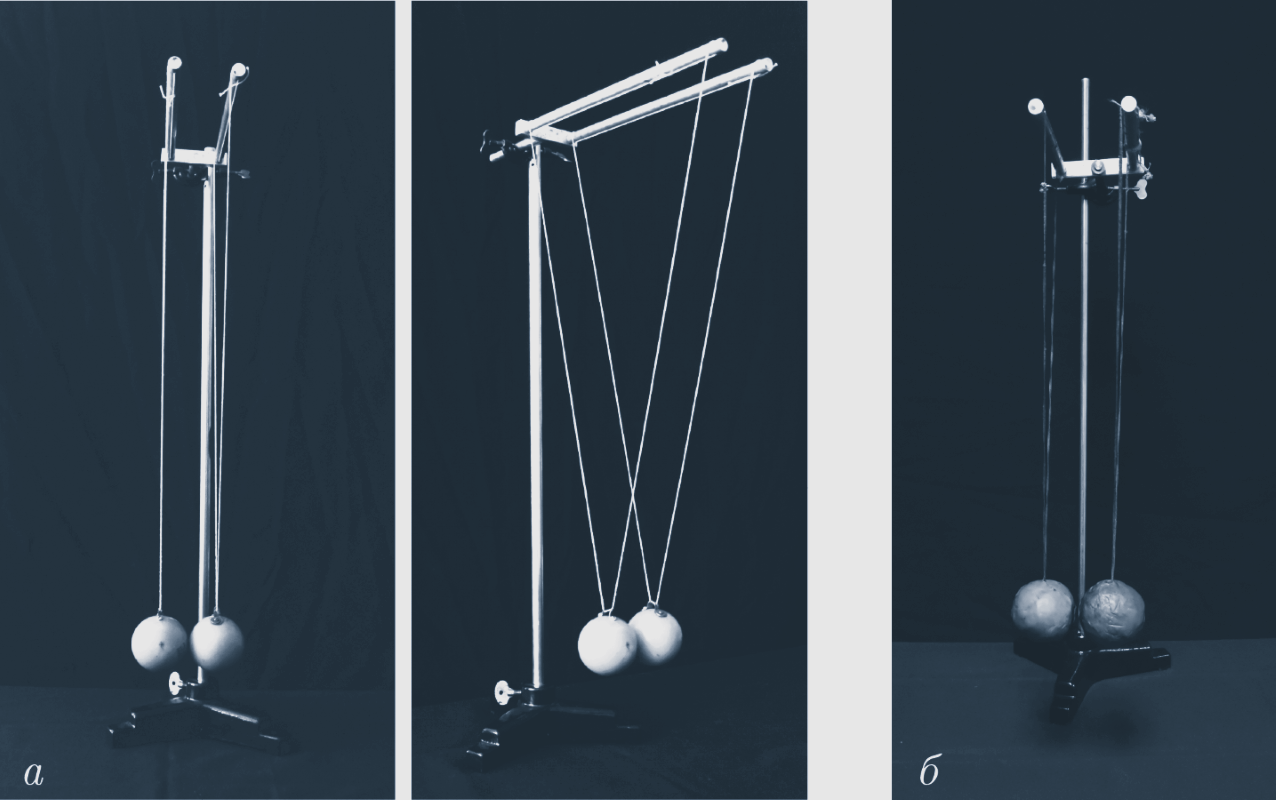
\includegraphics[width=0.9\linewidth]{hit-1.png}
		\caption{Демонстрация сохранения импульса при центральном соударении двух тел: \textit{а} — бильярдные шары (удар — упругий); \textit{б} — пластилиновые шары (удар — неупругий)}
		\label{hit-1}
	\end{figure}
	
	\subsection*{\underline{Оборудование:}}
	
	\begin{enumerate} 
		\item Пара бильярдных шаров на бифилярных подвесах 
		\item Пара шаров из пластилина с деформируемой поверхностью
		\item Специальный подвес
		\item Штатив
	\end{enumerate}

	\newpage
	\subsection*{\underline{Основные определения:}}
	
	Второй закон Ньютона в импульсной форме для системы материальных точек имеет вид
	$$
	\textbf{F}_{\text{внеш}} = \dfrac{d\textbf{P}}{dt},
	$$
	где $ \textbf{F}_{\text{внеш}} $ — результирующая внешних сил, действующих на систему, $\textbf{P}=\textbf{p}_1+\textbf{p}_2+\ldots+\textbf{p}_N$ — суммарный импульс системы \textit{N} тел. 
	
	Система тел называется замкнутой, если действия внешних тел на тела данной системы
	или пренебрежимо малы, или компенсируют друг друга.
	Таким образом, в случае замкнутой системы тел существенно 
	лишь взаимодействие этих тел друг с другом, но не с какими-либо
	другими телами.
	Равнодействующая внешних сил, приложенных к замкнутой системе, равна нулю: $ \textbf{F}_{\text{внеш}}=0 $.
	В этом случае $$ \dfrac{d\textbf{P}}{dt} =0.$$
	Если производная по времени или, другими словами, скорость изменения импульса \textbf{P} обращается в нуль, то сам вектор не меняется со временем, т. е. сохраняется: $ \textbf{P}= \text{const}$.
	Закон сохранения импульса можно сформулировать в следующем виде:
	\textit{\begin{flushleft}
			Импульс замкнутой системы тел остается постоянным с течением времени при любых взаимодействиях тел внутри данной системы.
	\end{flushleft}}

При соударении двух тел удар называется прямым и центральным, когда общая нормаль к поверхностям тел в точке касания проходит через их центры масс и когда скорости центров масс в начале удара направлены по этой общей нормали.
Таким, в частности, будет удар двух однородных шаров, центры которых до удара движутся вдоль одной и той же прямой. 
		
	\newpage
	\subsection*{\underline{Краткое описание:}}
	
	Для демонстрации закона сохранения импульса на примере системы из двух подвесных маятников вначале необходимо подобрать длину нитей такой, чтобы соударение тел было центральным.
	
	В ходе опыта с двумя бильярдными шарами одинаковой массы, отклонив один из шаров, отпускают его (рис.\ref{hit-2},\textit{а}).
	Под действием силы тяжести этот шар начнет изменять скорость, а, следовательно до столкновения с покоящимся телом, его успеет приобрести некоторый импульс (рис.\ref{hit-2},\textit{б}).
	Ударившись о второй шар, первый останавливается, а второй отклоняется почти на такое же расстояние, на какое был отклонен первый (рис.\ref{hit-2},\textit{в}). 
	Затем второй шар ударится о первый и останется на месте, а первый шар отклонится и т. д.
	После трех-пяти ударов шары следует остановить, т. к. вследствие не вполне упругого удара они оба приходят в движение.
		
	\begin{figure}[H]
			\centering	
			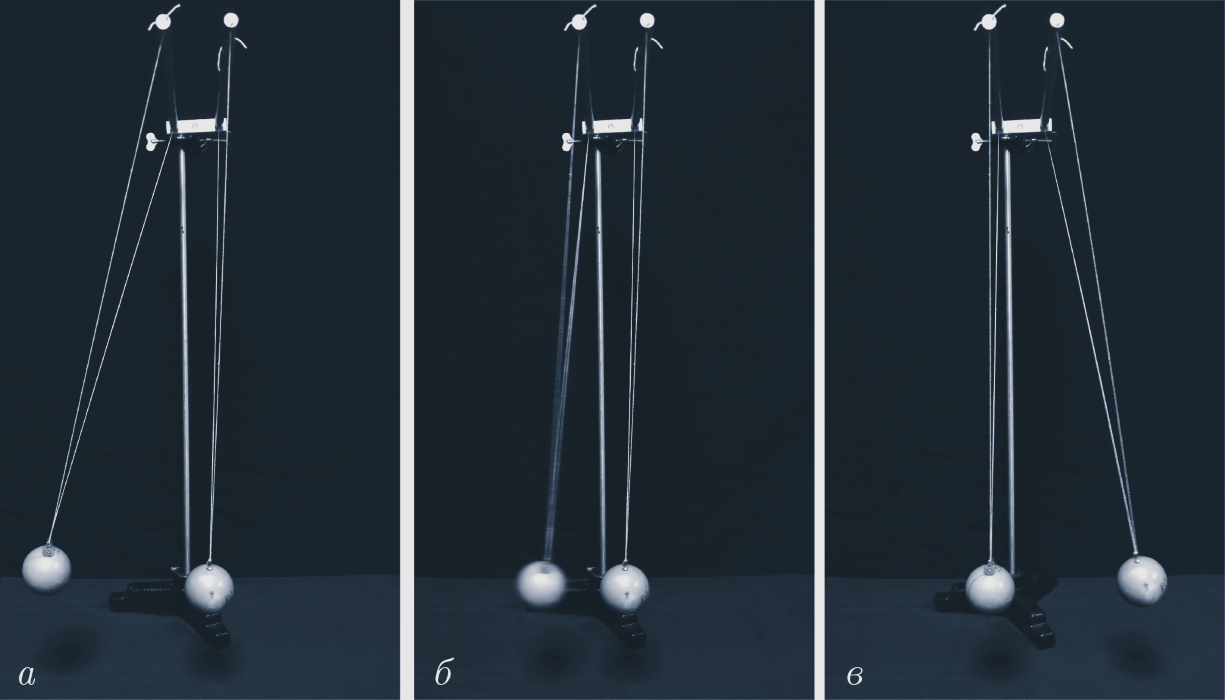
\includegraphics[width=0.9\linewidth]{hit-2.png}
			\caption{Демонстрация сохранения импульса при упругом ударе. Если отклонить один из шаров на некоторый угол и отпустить, то после столкновения этот шар остановится, а второй отклонится на тот-же угол}
			\label{hit-2}
		\end{figure}

Для следующей демонстрации, которая позволяет пронаблюдать закон сохранения импульса при неупругом ударе, т. е. в случае, когда при столкновении двух тел существенным оказывается их деформация, на штатив подвешиваются два пластилиновых шара одинакового размера и массы.
В положении равновесия пластилиновые шары слегка касаются друг друга.

	\begin{figure}[H]
	\centering	
	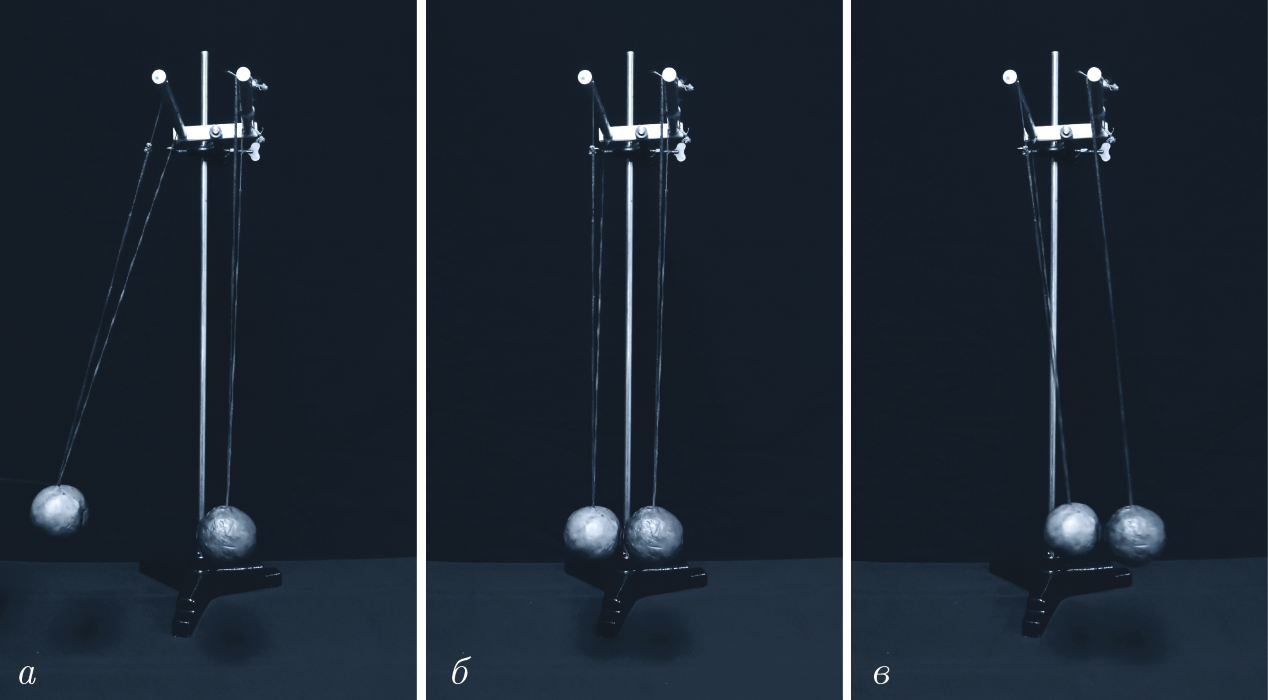
\includegraphics[width=0.9\linewidth]{hit-3.png}
	\caption{Демонстрация сохранения импульса при неупругом соударении шаров. В момент удара тела деформируются, часть импульса теряется, а объединившиеся в результате столкновения шары отклоняются на меньший угол}
	\label{hit-3}
\end{figure}

Такая система по-прежнему является замкнутой, а, значит, для нее также справедлив закон сохранения импульса.
При отведении одного из шаров в сторону его отпускают.
после удара оба шара движутся совместно с одинаковой скоростью, но отклоняются на угол, меньший по сравнению с углом отклонения первого шара (рис.\ref{hit-3},\textit{а}).
Перед опытом один из шаров следует разогреть, усилив тем самым процесс слипания в момент удара.

Рассчитать скорость шаров после неупругого взаимодействия (рис.\ref{hit-3},\textit{в}), а также вычислить угол отклонения двух шаров можно при помощи закона сохранения импульса.

\newpage
\subsection*{\underline{Теория:}}

Закон сохранения импульса позволяет рассчитывать скорости сталкивающихся тел при абсолютно упругом или неупругом ударе.

\textit{Упругий удар.}
Рассмотрим изолированную систему, состоящую из двух тел.
С целью упрощения выкладок возьмем тела равной массы \textit{m}.
Пусть в некоторый момент времени эти тела имеют скорости $ \textbf{v}_1 $ и  $ \textbf{v}_2 $ и в течение 
времени $ \Delta t $ действуют друг на друга с некоторыми силами $ \textbf{F}_1 $ и $ \textbf{F}_2 $.
Определим, как будут связаны друг с другом скорости $ \textbf{u}_1 $ и $ \textbf{u}_2 $, которые приобретут 
тела после такого взаимодействия.

Пренебрегая сопротивлением воздуха, систему можно считать замкнутой.
Поэтому для нее будет справедлив закон сохранения импульса:
	\begin{equation}\label{hit-1eq1}
\textbf{p}_{\text{до}}  = \textbf{p}_{\text{после}}.
\end{equation}

Импульс системы до удара — это сумма импульсов тел:
	\begin{equation}\label{hit-1eq2}
\textbf{p}_{\text{до}}  = m \textbf{v}_1 + m \textbf{v}_2.
\end{equation}
Для наглядности опыта одно из тел в начале можно рассмотреть неподвижным, т. е. его скорость $ \textbf{v}_1 $ до столкновения следует принять равной нулю (рис.\ref{hit-4},\textit{а}).
Полный импульс системы в этом случае складывается только из импульса второго шара, который до момента столкновения успевает приобрести скорость $ \textbf{v}_2 $ (рис.\ref{hit-4},\textit{б}).


\begin{figure}[H]
	\centering 	
	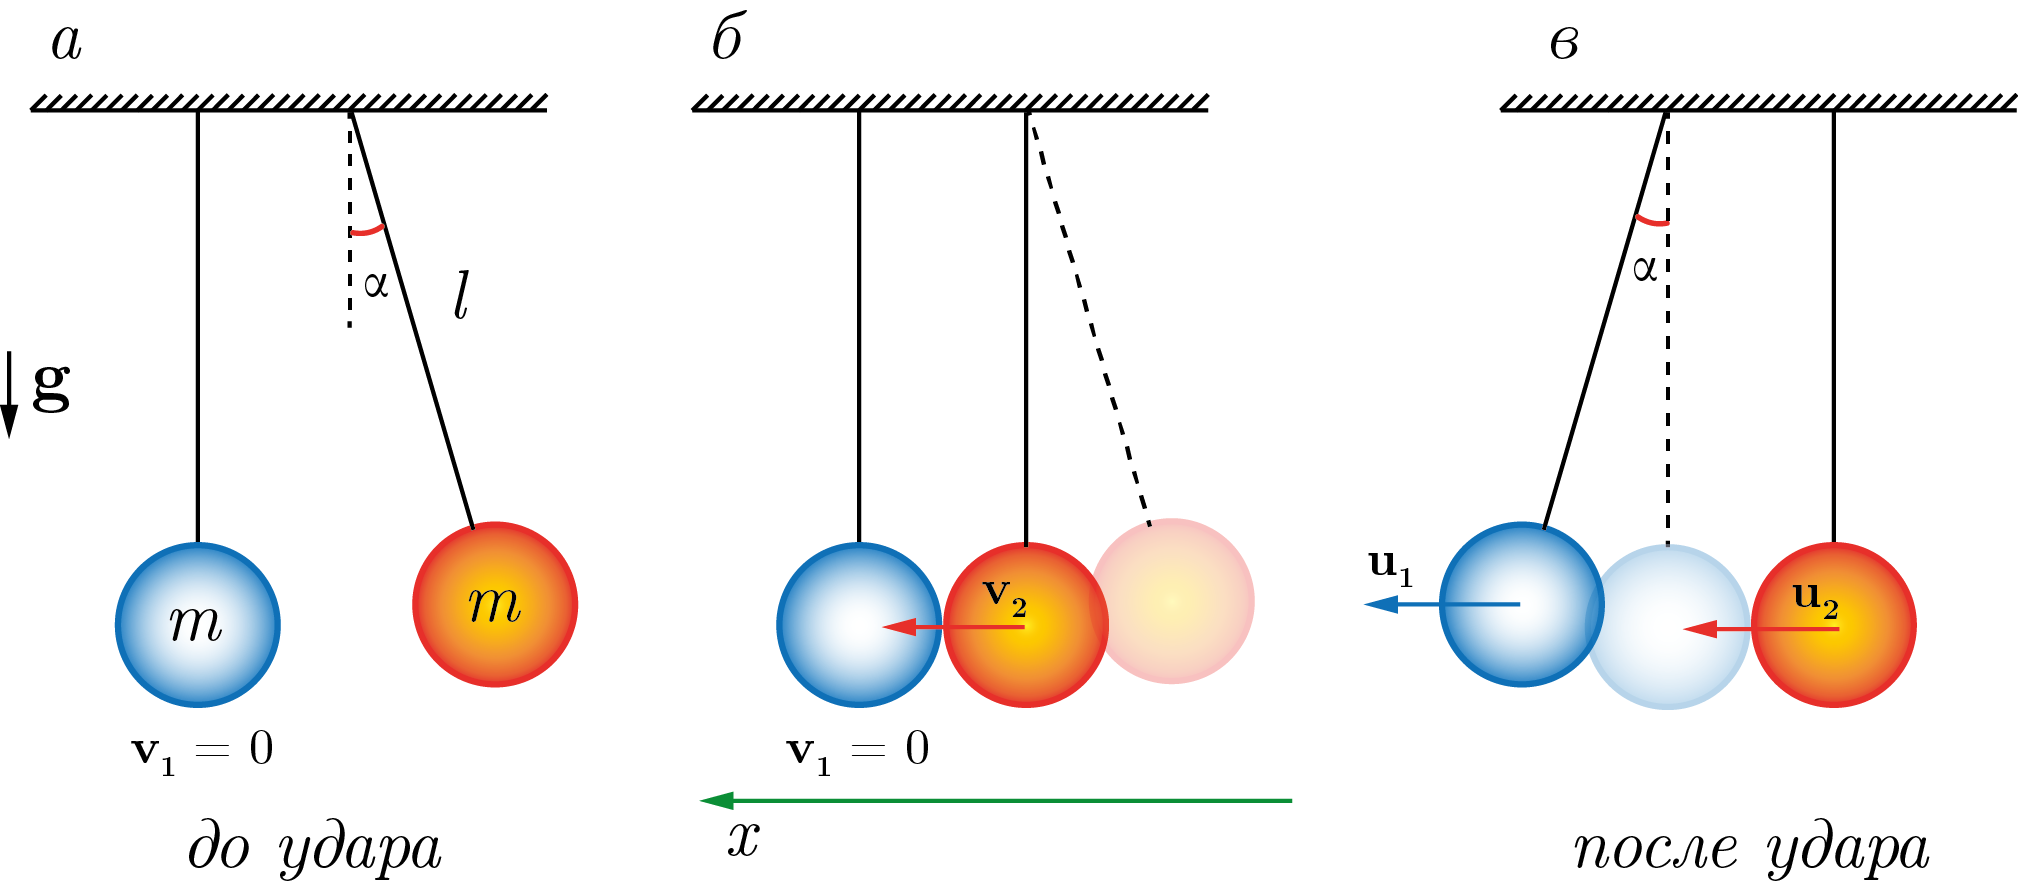
\includegraphics[width=0.9\linewidth]{hit-4.png}
	\caption{При упругом столкновении двух шаров одинаковой массы импульс тела $ p=mv_2 $ полностью передается покоящемуся шару. После удара первый шар останавливается, а второй отклоняется на тот же угол}
	\label{hit-4}
\end{figure}

В момент упругого соударения тела взаимодействуют в течение промежутка времени $ \Delta t $ внутри системы происходит перераспределение импульса.
Неподвижный шар, испытывая действие силы со стороны ударяющего шара, приобретает ускорение, и в результате начинает движение в туже сторону, куда двигался второй шар (рис.\ref{hit-4},\textit{в}).
Передав в ходе взаимодействия часть импульса, движущийся шар замедлится.
После упругого соударения (без учета сопротивления воздуха и деформации шаров) полный импульс системы станет равным:

	\begin{equation}\label{hit-1eq3}
\textbf{p}_{\text{после}}  = m \textbf{u}_1 + m \textbf{u}_2.
\end{equation}

Из закона сохранения импульса имеем:
	\begin{equation}\label{hit-1eq4}
m \textbf{v}_1 + m \textbf{v}_2  = m \textbf{u}_1 + m \textbf{u}_2,
\end{equation}
или с учетом покоя в начальный момент одного из шаров ( $ \textbf{v}_1=0 $):
	\begin{equation}\label{hit-1eq5}
\textbf{v}_2  = \textbf{u}_1 + \textbf{u}_2.
\end{equation}

Из опыта следует, что при центральном упругом соударении шаров одинаковой массы, один из которых до удара покоится, импульс движущегося шара полностью передается неподвижному телу.
При этом первый шар останавливается, то есть его скорость после взаимодействия $ \textbf{u}_2=0 $.  
Из соотношения для скоростей (\ref{hit-1eq5}) тогда следует, что $ \textbf{u}_1  = \textbf{v}_2 $.
Другими словами, импульс одного из шаров ($ m\textbf{v}_2 $) при упругом взаимодействии полностью переходит другому шару, который начинает движение с той же самой скоростью.
Угол отклонения этого шара окажется равным начальному углу $ \alpha $.

\textit{Непругий удар.}
Задача о нахождении скорости тел после неупругого столкновения оказывается проще, чем для упругого удара, поэтому можно рассмотреть более общий случай столкновения двух тел различной массы  $ m_1 $ и  $ m_2 $.
Полный импульс системы до удара в этом случае также есть величина $$ \textbf{p}_{\text{до}}  = m_1 \textbf{v}_1 + m_2 \textbf{v}_2.$$
После неупругого соударения тела деформируются и слипаются, образуя тело массой $m = m_1 + m_2 $, которое начинает двигаться со скоростью \textbf{u} как единое целое (рис.\ref{hit-5},\textit{в}).

\begin{figure}[H]
	\centering 	
	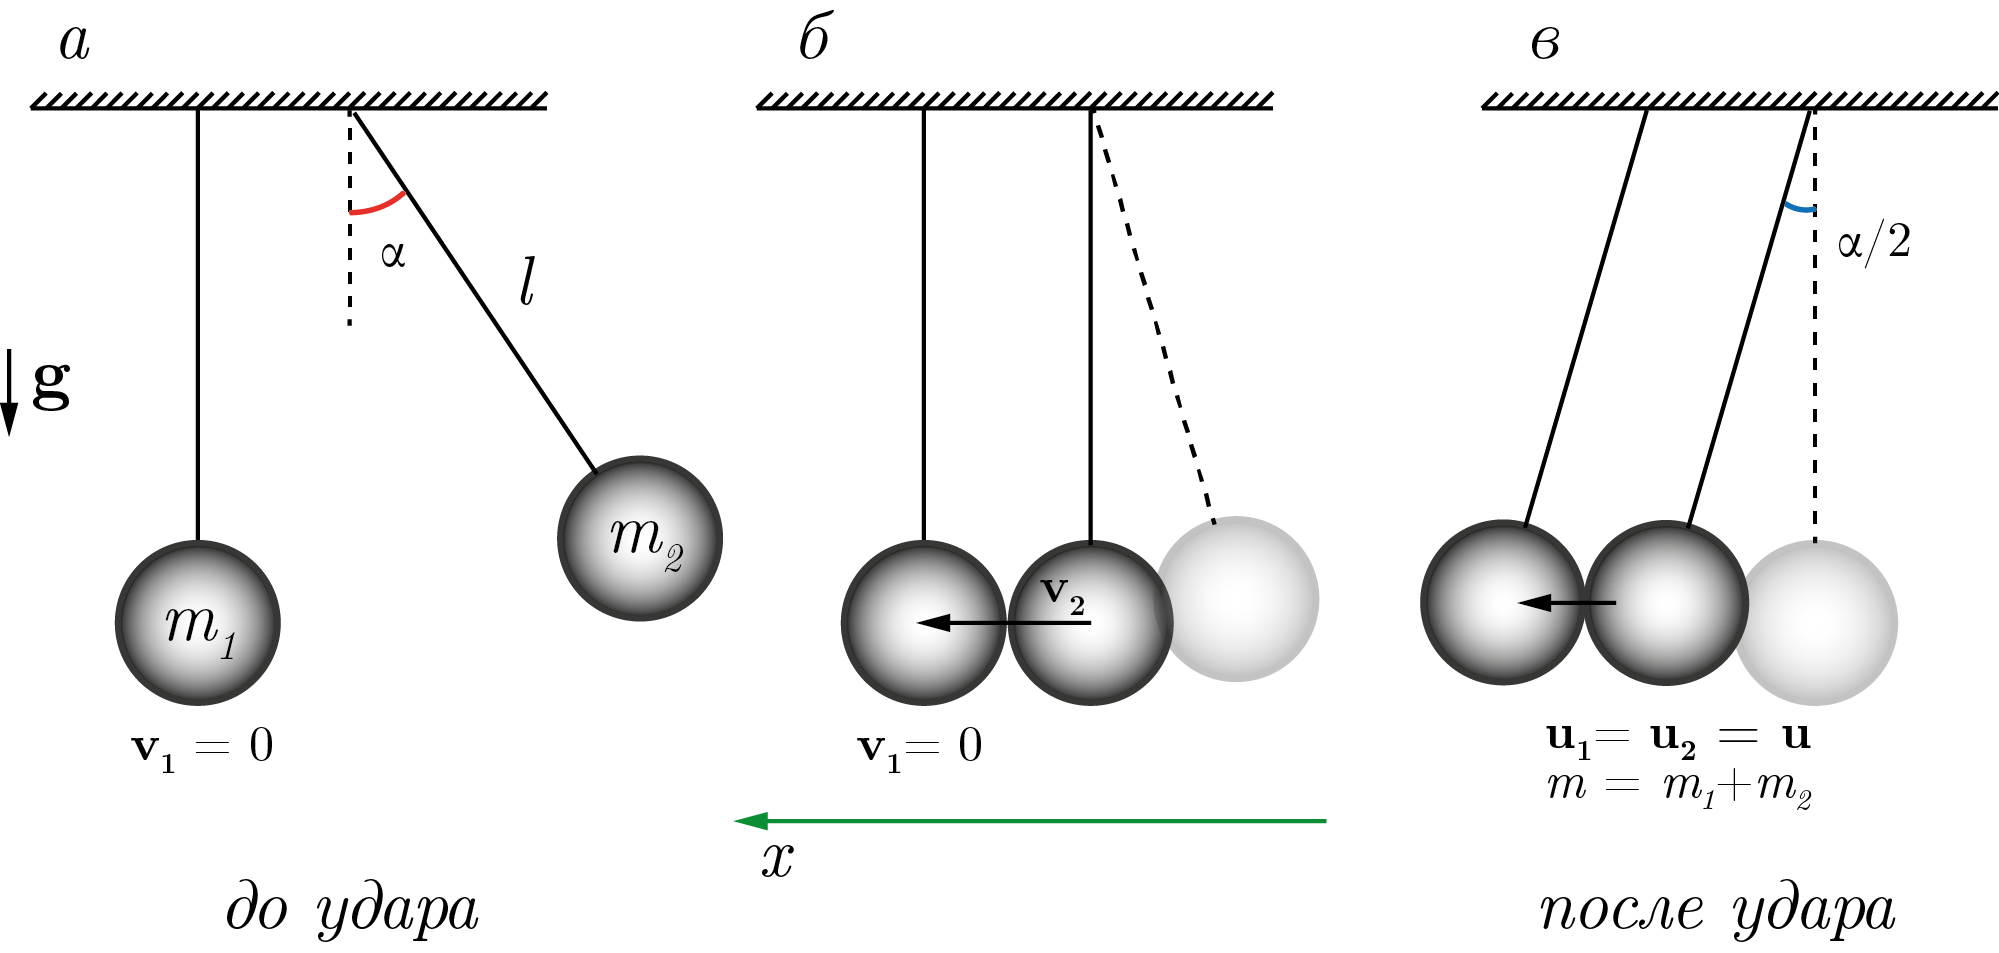
\includegraphics[width=0.9\linewidth]{hit-5.png}
	\caption{При неупругом столкновении двух шаров импульс одного из тел ($ p_2=m_2v_2 $) перераспределяется внутри системы из двух тел общей массой $ m= m_1 + m_2 $. После объединения шаров в единое целое скорость движения все системы в силу закона сохранения импульса уменьшится. Также станет меньше угол, на который отклонится вся система после взаимодействия}
	\label{hit-5}
\end{figure}

Импульс такой системы после соударения равен $$ \textbf{p}_{\text{до}}  = (m_1 + m_2) \textbf{u}.$$
Отсюда можно определить скорость системы после удара:
	\begin{equation}\label{hit-1eq6}
\textbf{u}  = \dfrac{m_1 \textbf{v}_1 + m_2 \textbf{v}_2}{m_1 + m_2}=\dfrac{m_1 \textbf{v}_1 + m_2 \textbf{v}_2}{m},
\end{equation}
или в проекции на горизонтальную ось \textit{x}:
	\begin{equation}\label{hit-1eq7}
u_x  = \dfrac{m_1 v_{1x} + m_2 v_{2x}}{m}.
\end{equation}

Для случая столкновения тел одинаковой массы (один из шаров по-прежнему в начале неподвижен, $ v_{1x}=0 $), скорость системы после взаимодействия будет равна половине начальной скорости, т.е. $ u_x = v_{2x}/2 $, причем их направления будут совпадать.
Вся система при этом отклониться на угол вдвое меньше начального угла, на который до удара был отклонен один из шаров.

\end{document}